\section{Carry handles}

\subsection{Motivation}
By the conclusion of the preproject, the sensor rig was portable, but it lacked ergonomic handles.
In the previous design required the user would have to hold on to the carbon fiber rods directly, which was uncomfortable and made it difficult to keep the sensor rig steady.
Moreover, the existing design relied on controlling the software via a mobile phone, which necessitated the use of one hand intermittently, rendering the previous design very impractical.
To address these issues, ergonomic carry handles were designed and subsequently 3D printed, providing enhanced comfort and usability.


\subsection{Grip design}
First the grip was designed, which is the part that the user holds on to.
Initially, it was recognized that developing an ergonomic handle from scratch would be a demanding and time-consuming task, given the intricate geometric shapes necessary to ensure a comfortable fit in the human hand.
Consequently, the decision was made to find an existing design to use as a starting point.
To find a suitable design, the following search terms and model sites were utilized:

\begin{multicols}{2}
    \textbf{3Dmodel sites}:
    \begin{itemize}
        \item Thingiverse
        \item Printables
        \item GrapCad
        \item Cults
        \item Free3D
    \end{itemize}
    \columnbreak
    \textbf{Key words:}:
    \begin{itemize}
        \item handle
        \item grip
        \item ergonomic handle
        \item ergonomic grip
        \item carry handle
        \item carry grip
    \end{itemize}
\end{multicols}


A set of well-designed ergonomic handles, with a permissive license, was ultimately discovered on Printables \cite{matulichErgonomicHandleBased}.
The handles were meticulously documented on the creator's blog page \cite{matulichWhoseHandsAre2022}, taking into consideration the anatomy of the human hand.
The selected model featured well designed finger grooves, providing a solid foundation for a comfrtable carry handle.



However, as the model did not fit my hands perfectly, several iterations were undertaken to achieve a better fit.
To determine the appropriate scaling, the grip's outline was printed in multiple sizes using "vase mode," a technique where the printer creates a continuous spiral outline of the model for quick iteration \cite{ghargeCuraVaseMode2022}.
One of these test prints is shown in Figure \ref{fig:handle_iteration}.

\begin{figure}[H]
    \centering
    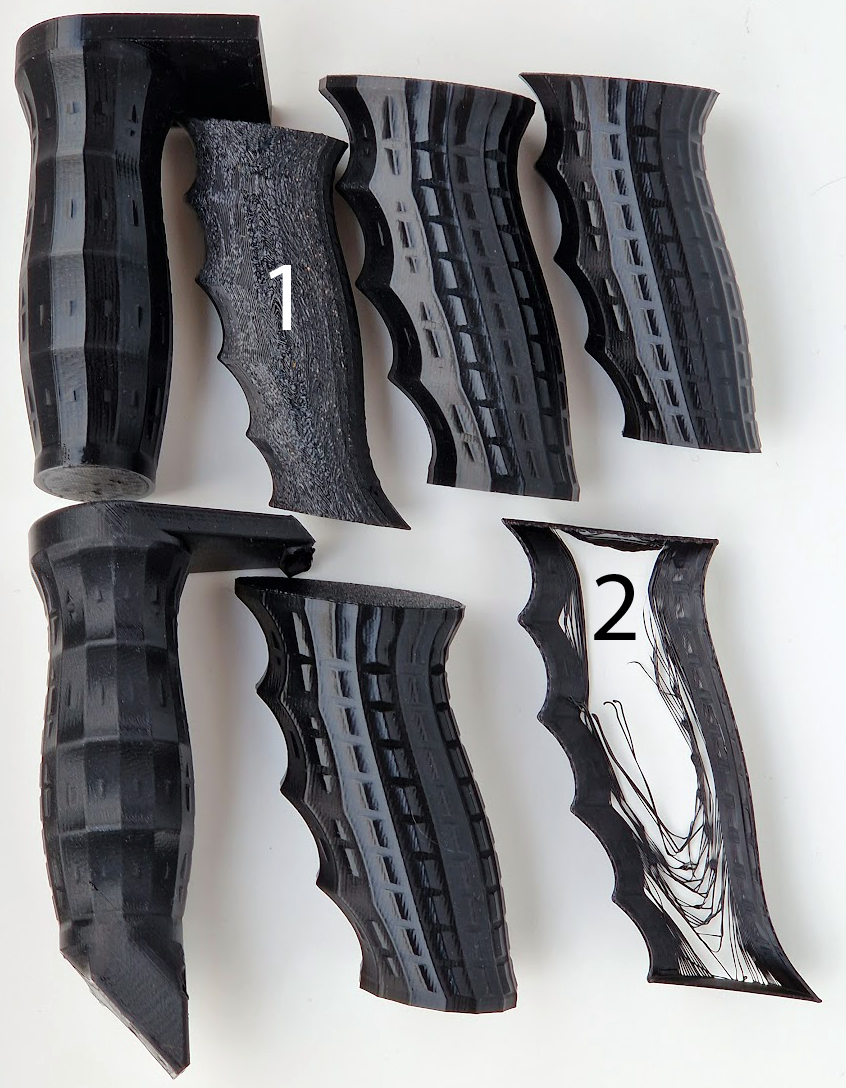
\includegraphics[width=.5\textwidth]{figures/3d_print/handles.png}
    \caption{Iterations on carry handle design.
        The handle marked with a 1 was printed sideways, resulting in a bad underside.
        The handle marked with a 2 shows one of the many handles printed in "vase mode" for fast iteration.}
    \label{fig:handle_iteration}
\end{figure}



After determining a rough size, the complete grip was printed in several different sizes, and a blind test was conducted with myself and a few friends to identify the best fit.
With our eyes closed, we held various grips and provided feedback on whether they felt too big, too small, or just right in each dimension.
To ensure consistency, the same grip was presented to each test subject multiple times.
Using the test results, the final design was adjusted to be 10\% taller, 20\% wider, and 25\% deeper compared to the original design.

\subsection{Integration with the sensor rig}
After the grip was finalized, they served as a stargin point for the desing of the carry handles.
The main goals were to have the grips positioned with an inclination matching the natural inclination of the hand, and keep them close to the center of gravity of the \sr to make the sensor rig as ergonomic as possible.

The design process leveraged the existing cad model of the sensor rig, which included the cad model of the center enclosure.
The center enclosure have slightly tilted sides, probablby to be injection molded, which made the deign of the carry handle more challenging \cite{booplaEnclosure}.

\begin{figure}[H]
    \centering
    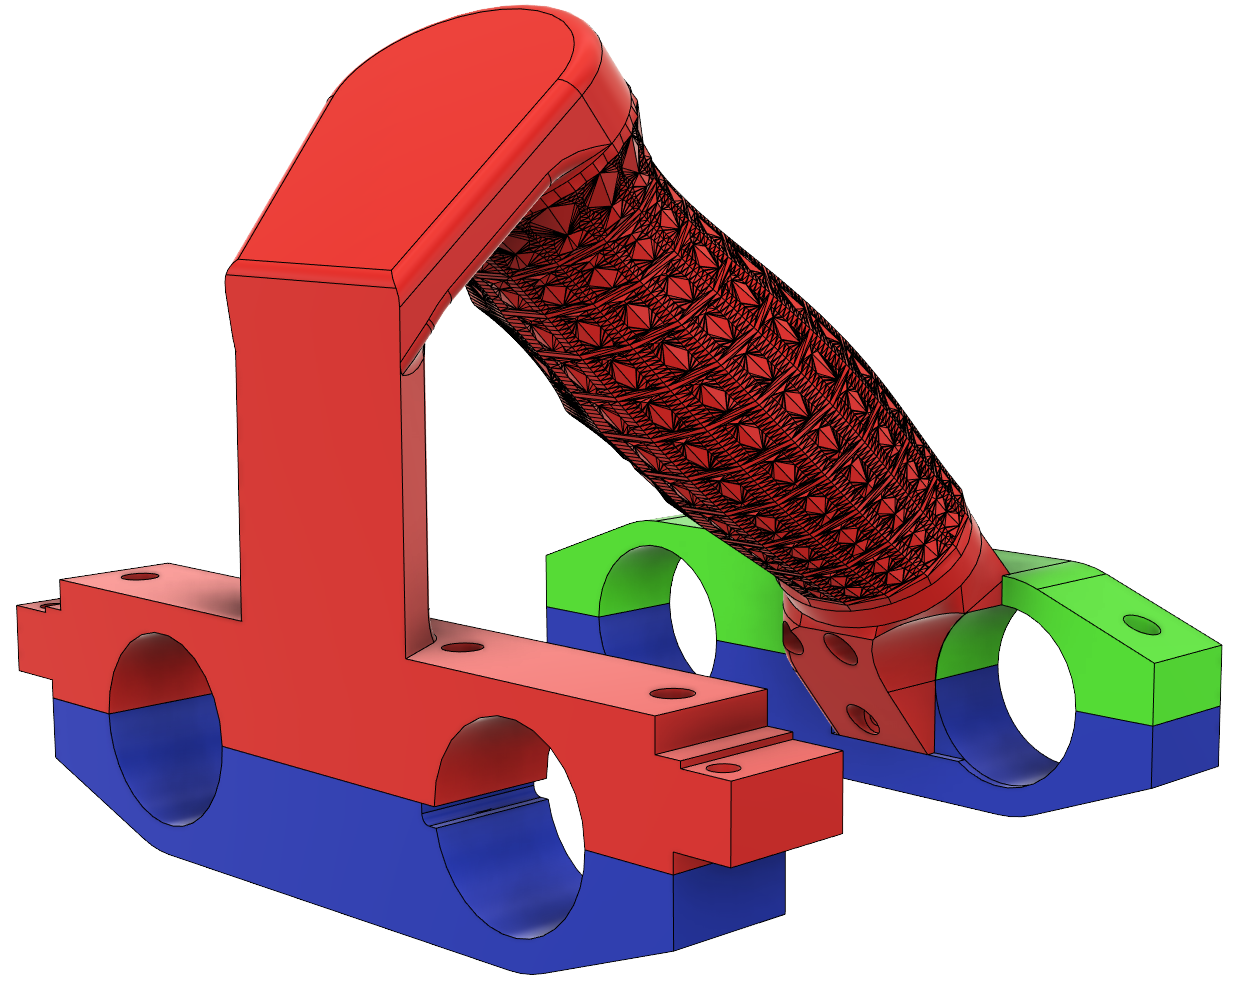
\includegraphics[width=.48\textwidth]{figures/3d_print/handle_cad.png}
    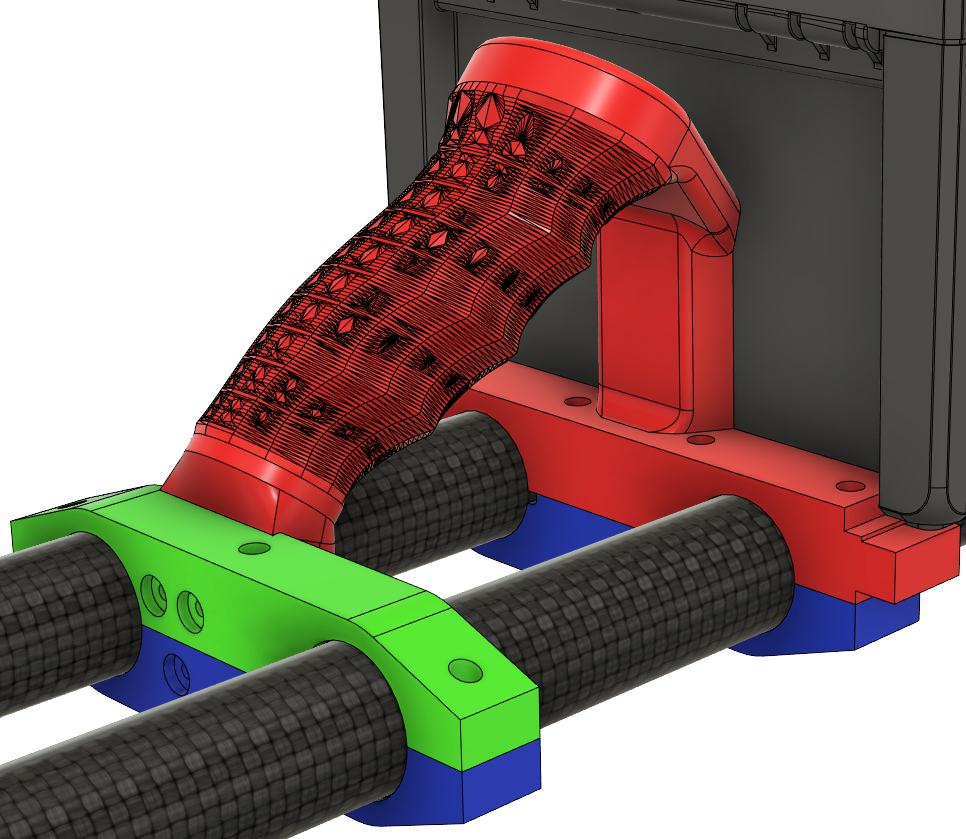
\includegraphics[width=.48\textwidth]{figures/3d_print/handle_cad_2.png}
    \caption{\gls{cad} model of the carry handle with constituent parts highlighted in different colors.}
    \label{fig:constituent_parts}
\end{figure}

The carry handles are made up of four constituent parts, as shown in Figure \ref{fig:constituent_parts}.
Initially the whole upper half was designed as a single part (red and green), but this reaulted in a failed prints due to too much overhang, as shown in Figure \ref{fig:handle_fail}.
With a better break-away support filament this might have been possible, but splitting the part seemd like a better option.
In the current design three M3 screws are used to attach the grip to the secon pair of tube clamps, ensuring a solid connection.
Multiple iterations were made to determine the optimal position and angle of the grips, aiming to achieve maximum comfort during handling.
A final touch was to add a small notch to the bottom clamp, for the \gls{gnss} antenna cable to pass through.

\begin{figure}[H]
    \centering
    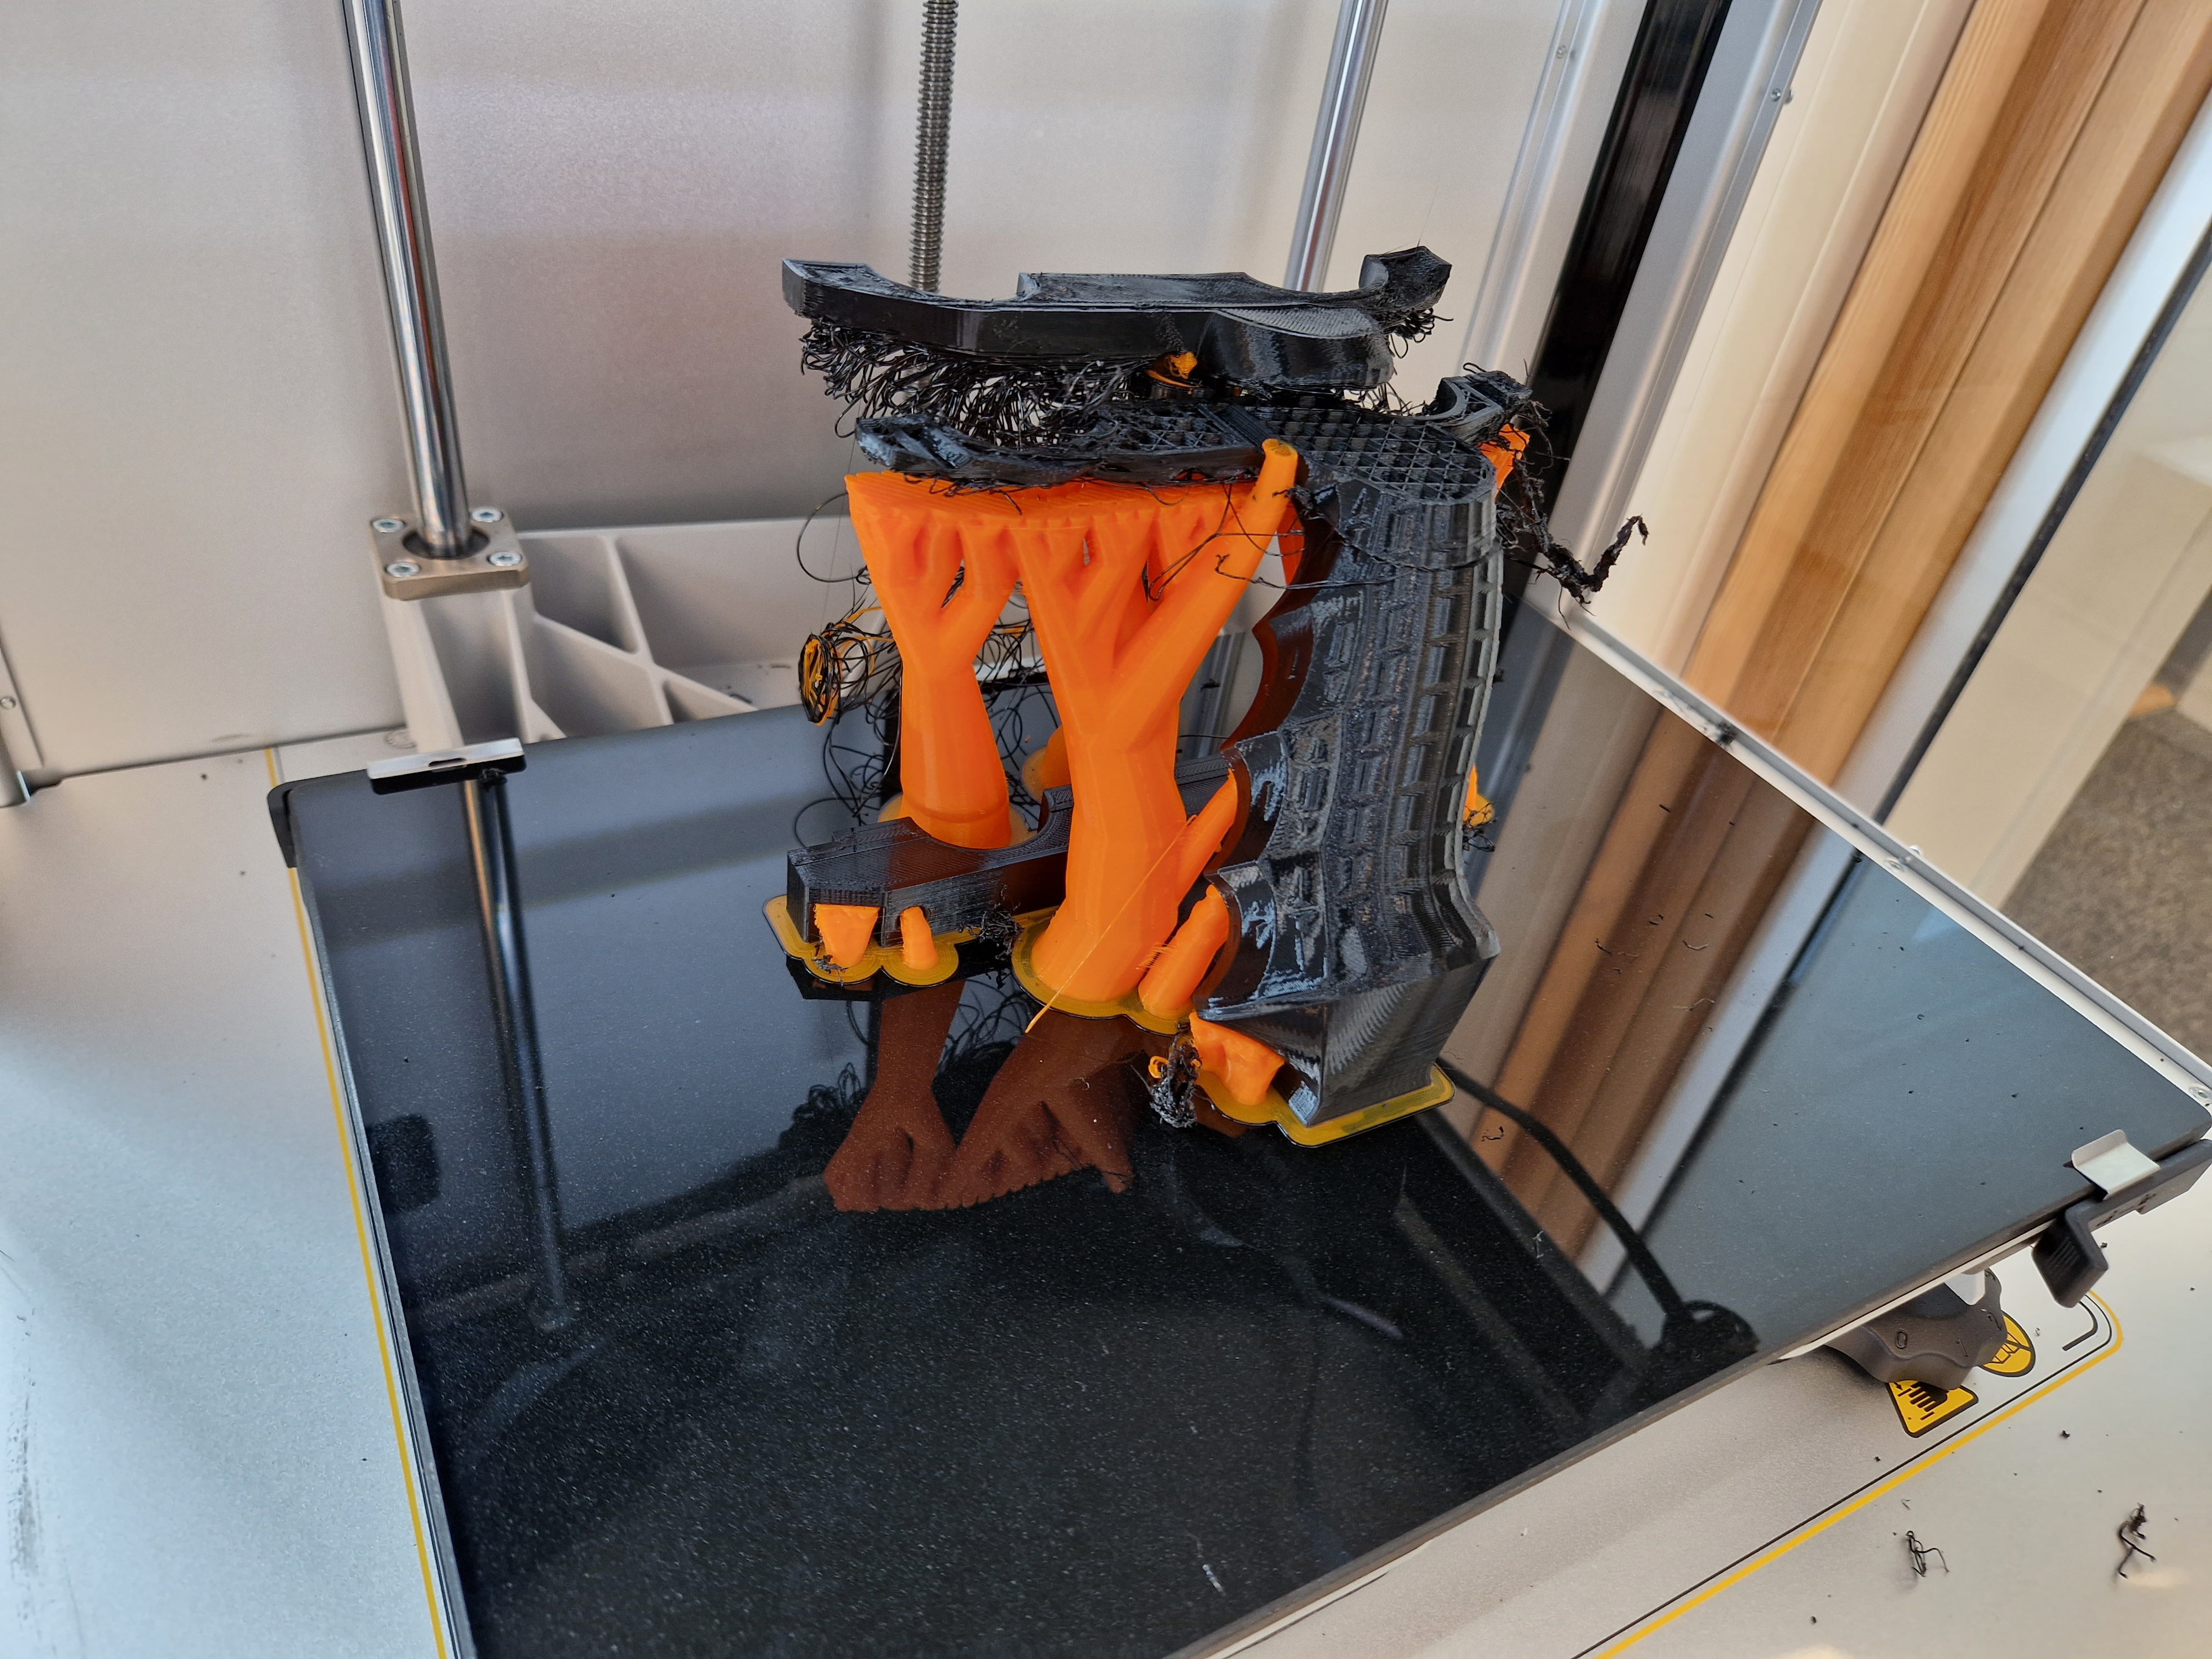
\includegraphics[width=.6\textwidth]{figures/3d_print/failed.jpg}
    \caption{Failed print when printing the whole upper part of the carry handle in one go, due to too much overhang.}
    \label{fig:handle_fail}
\end{figure}


\subsection{Durability}
The first iteration of the carry grips were possible to break by hand, and where thus not deemed solid enough.
To increase the durability, areas around the point of failure were thickened as shown in Figure \ref{fig:handle_thickness}, the wall thickness was increased to $3mm$ and infill increased to $40$.
The new carry grips were not possible to break by hand, and were deemed durable enough for the application.

\begin{figure}[H]
    \centering
    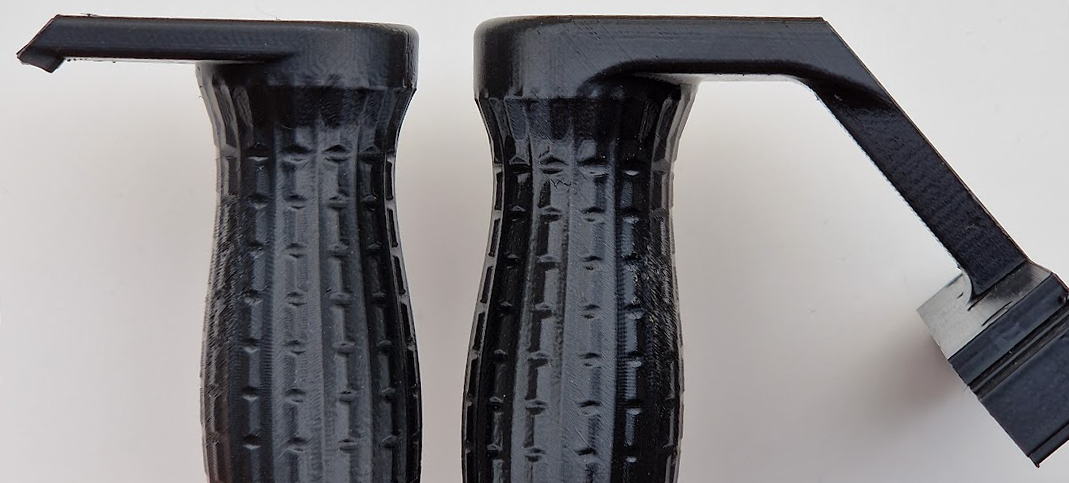
\includegraphics[width=.6\textwidth]{figures/3d_print/thickness.png}
    \caption{Initial and final iteration of carry handle.}
    \label{fig:handle_thickness}
\end{figure}

\subsection{Ergonomics}
The final carry handles have acieved the goals of providing an ergonomic way to hold the \sr.
With an inward inclination of $45^{\circ}$, the handles are positioned in a natural way, as shown in Figure \ref{fig:egonomics_a}.
The center enclosure have been moved slightly to the side, which makes space to hold the \sr easily with the left hand, using the elbow as counter balance as shown in Figure \ref{fig:egonomics_b}, which leaves the right hand available for fetching a phone from the pocket or perform other tasks.
If the operator desire to monitor the video feed it is easily acheived by resting the \sr on right forearm as shown in Figure \ref{fig:egonomics_c}.
The current design also have a lot of ground clearance to the ground when carried in a relaxed left hand as shown in Figure \ref{fig:egonomics_d}, which is usefull for transport.

\begin{figure}[H]
    \centering
    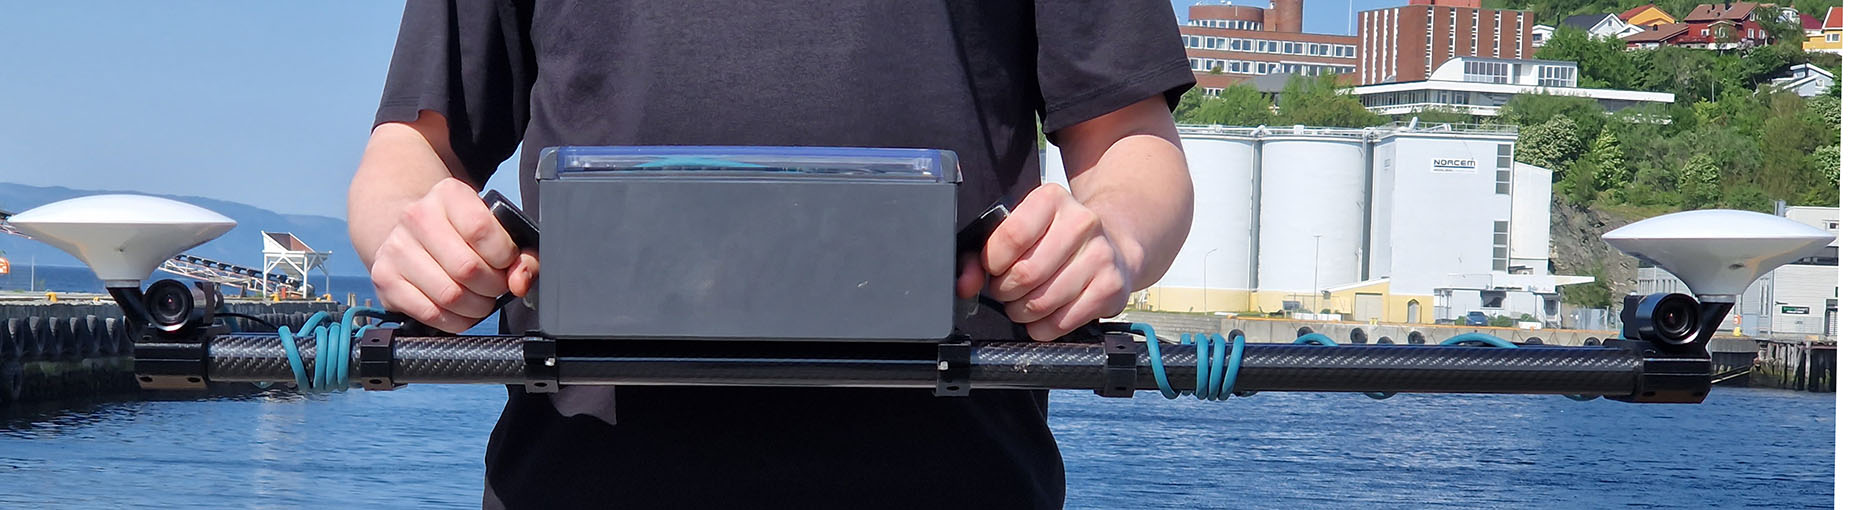
\includegraphics[width=\textwidth]{figures/ergonomics/dual_from_front.jpg}
    \caption{Demonstration of ergonomic two-handed grip.}
    \label{fig:egonomics_a}
\end{figure}
\begin{figure}[H]
    \centering
    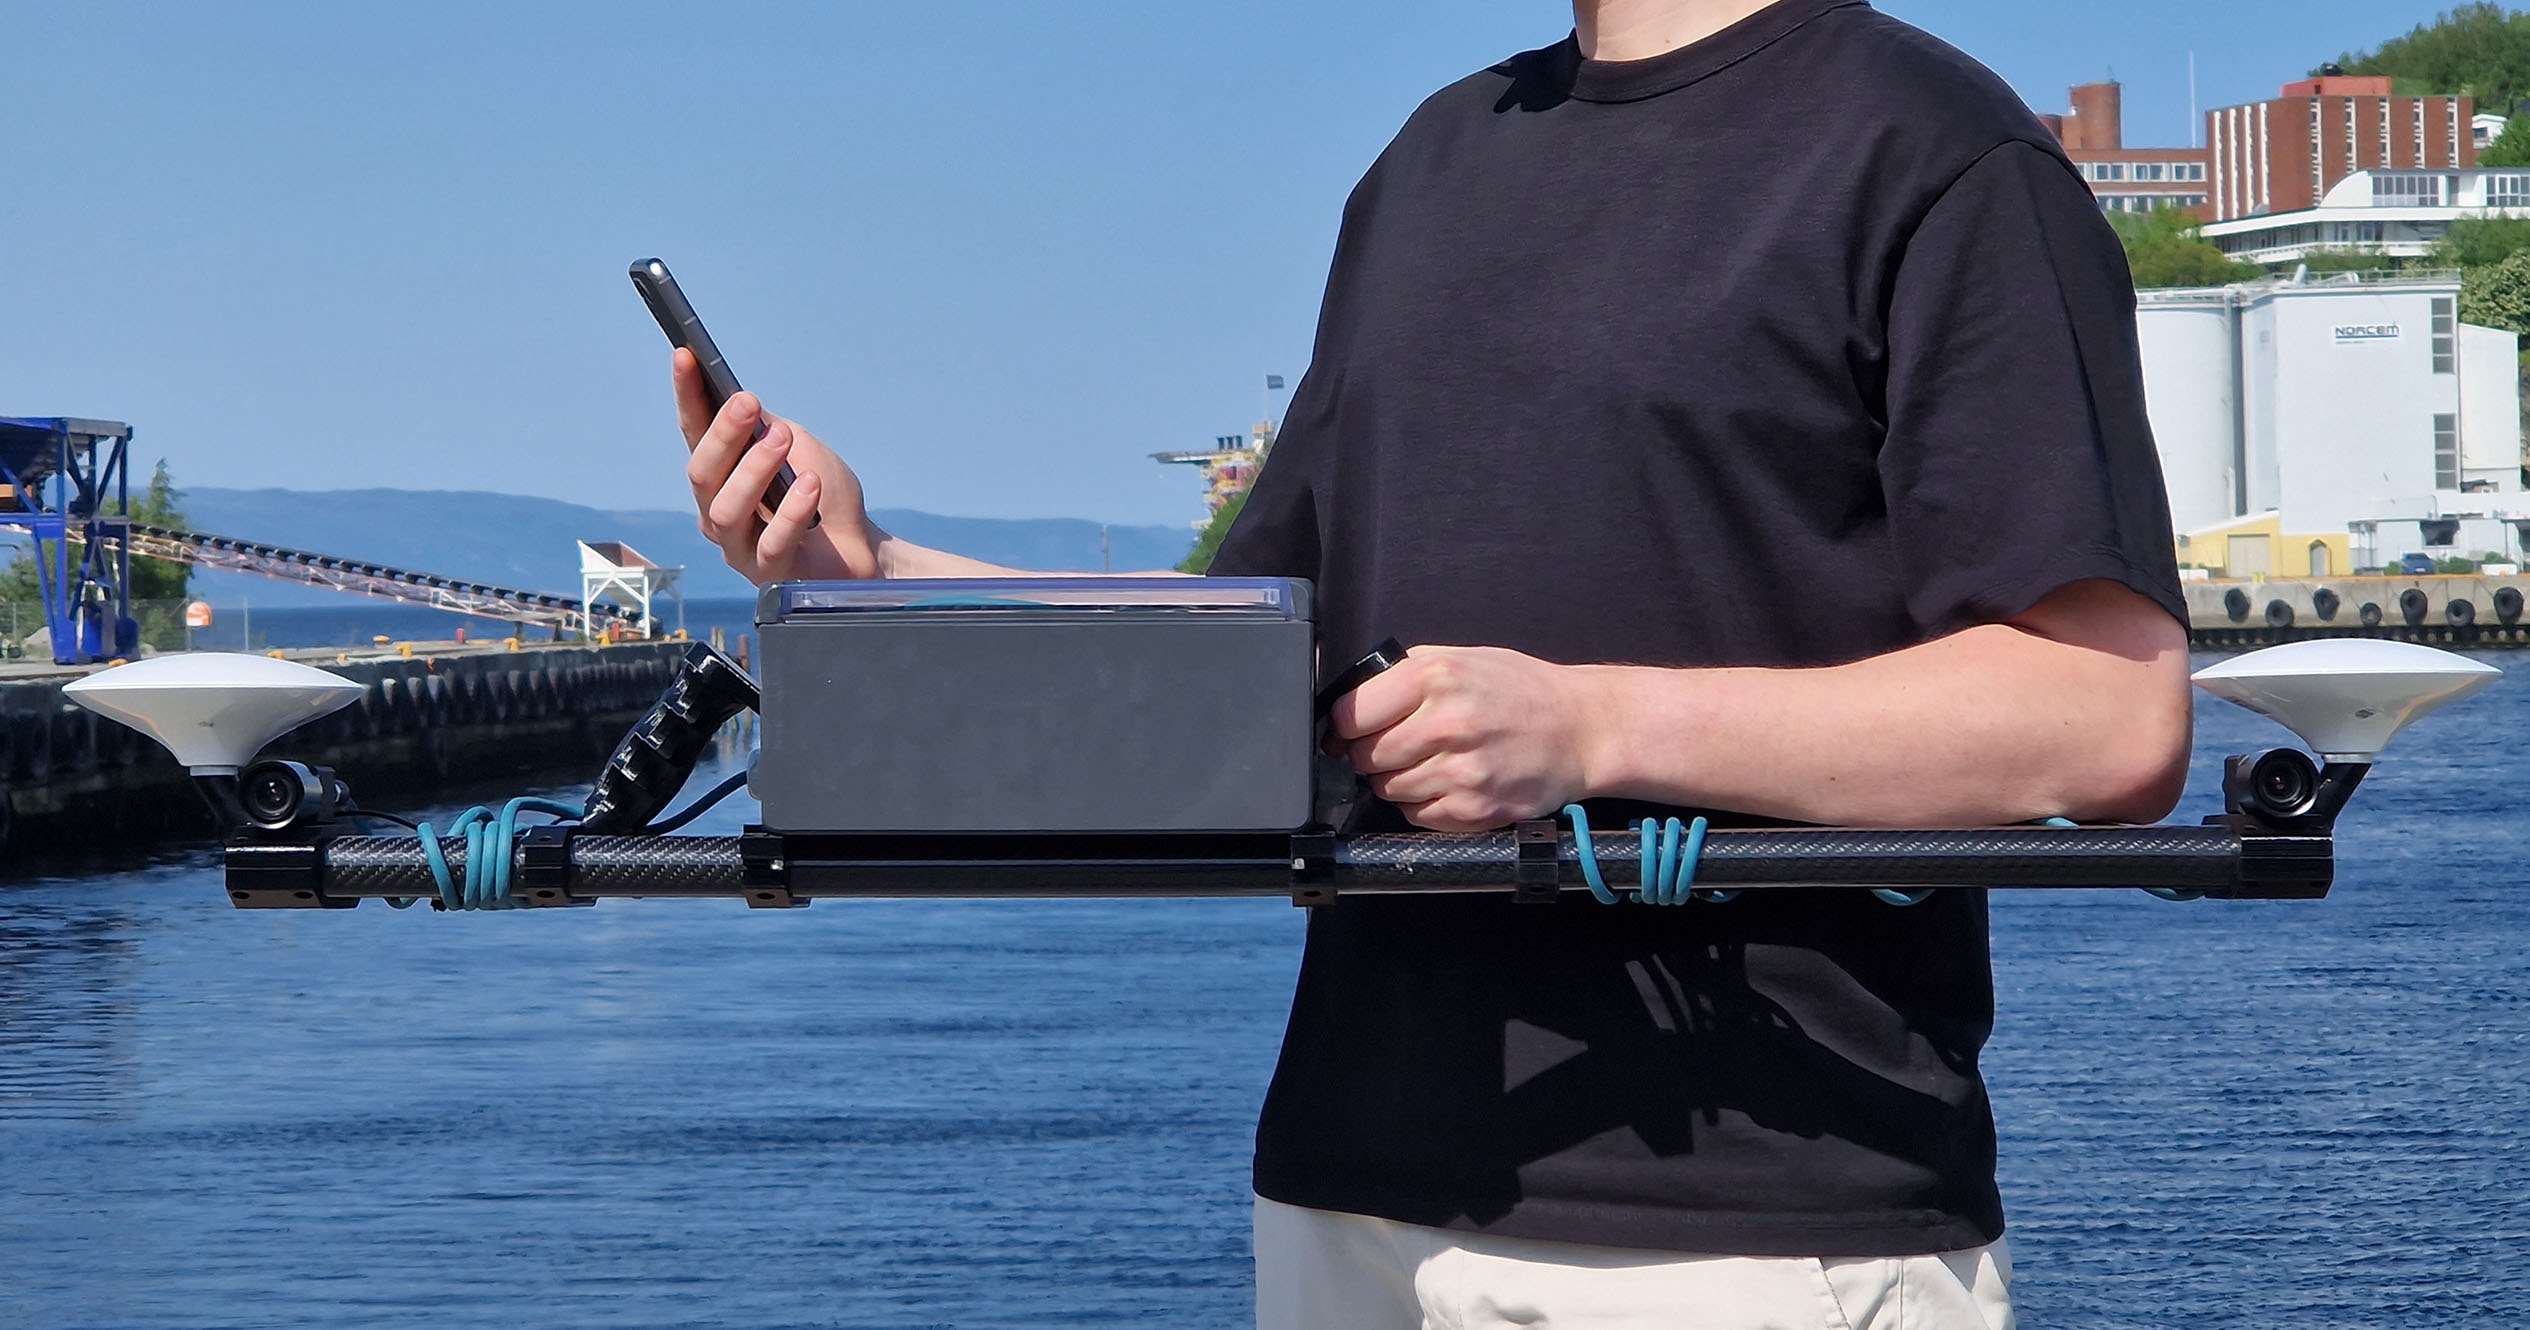
\includegraphics[width=\textwidth]{figures/ergonomics/single_hand.jpg}
    \caption{Photo showing how the \sr can easily be carried in the left hand, leaving the right hand free for other tasks.}
    \label{fig:egonomics_b}
\end{figure}
\begin{figure}[H]
    \centering
    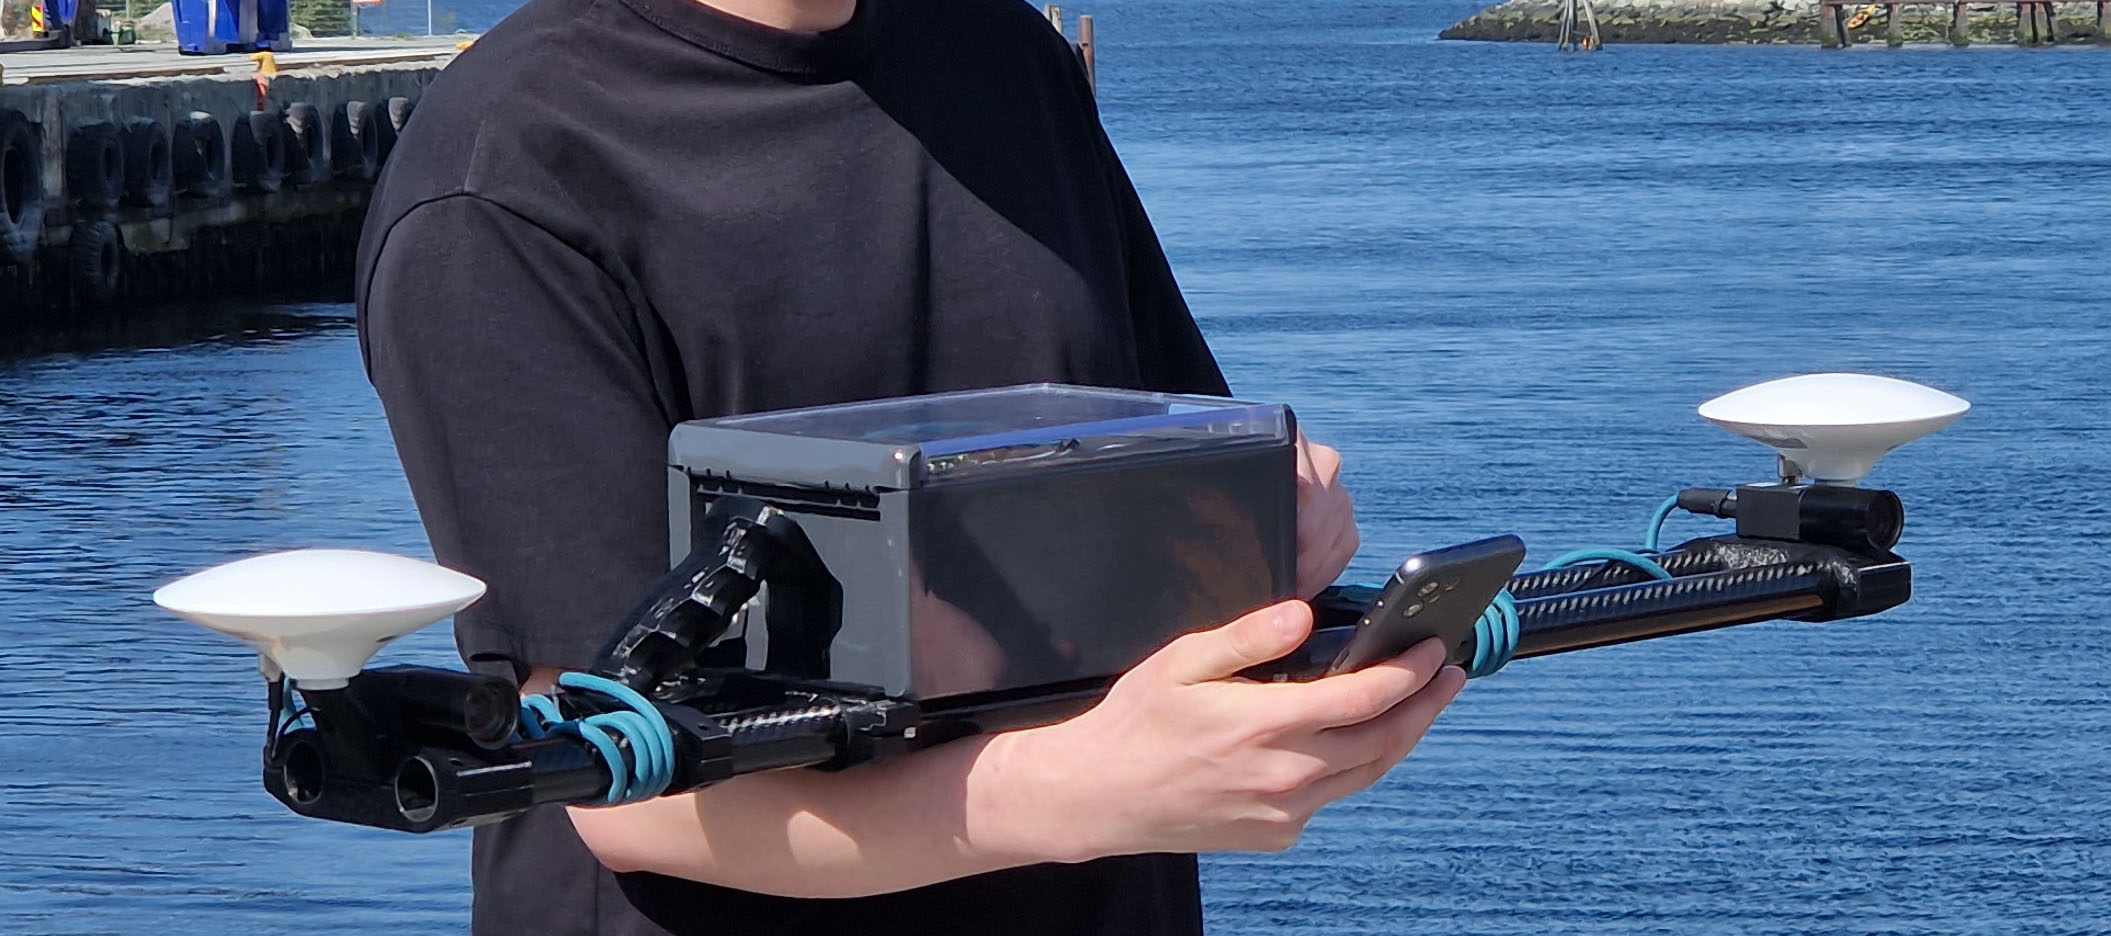
\includegraphics[width=\textwidth]{figures/ergonomics/holding_phone.jpg}
    \caption{Photo during operation of the \sr while video is monitored through a phone.}
    \label{fig:egonomics_c}
\end{figure}
\begin{figure}[H]
    \centering
    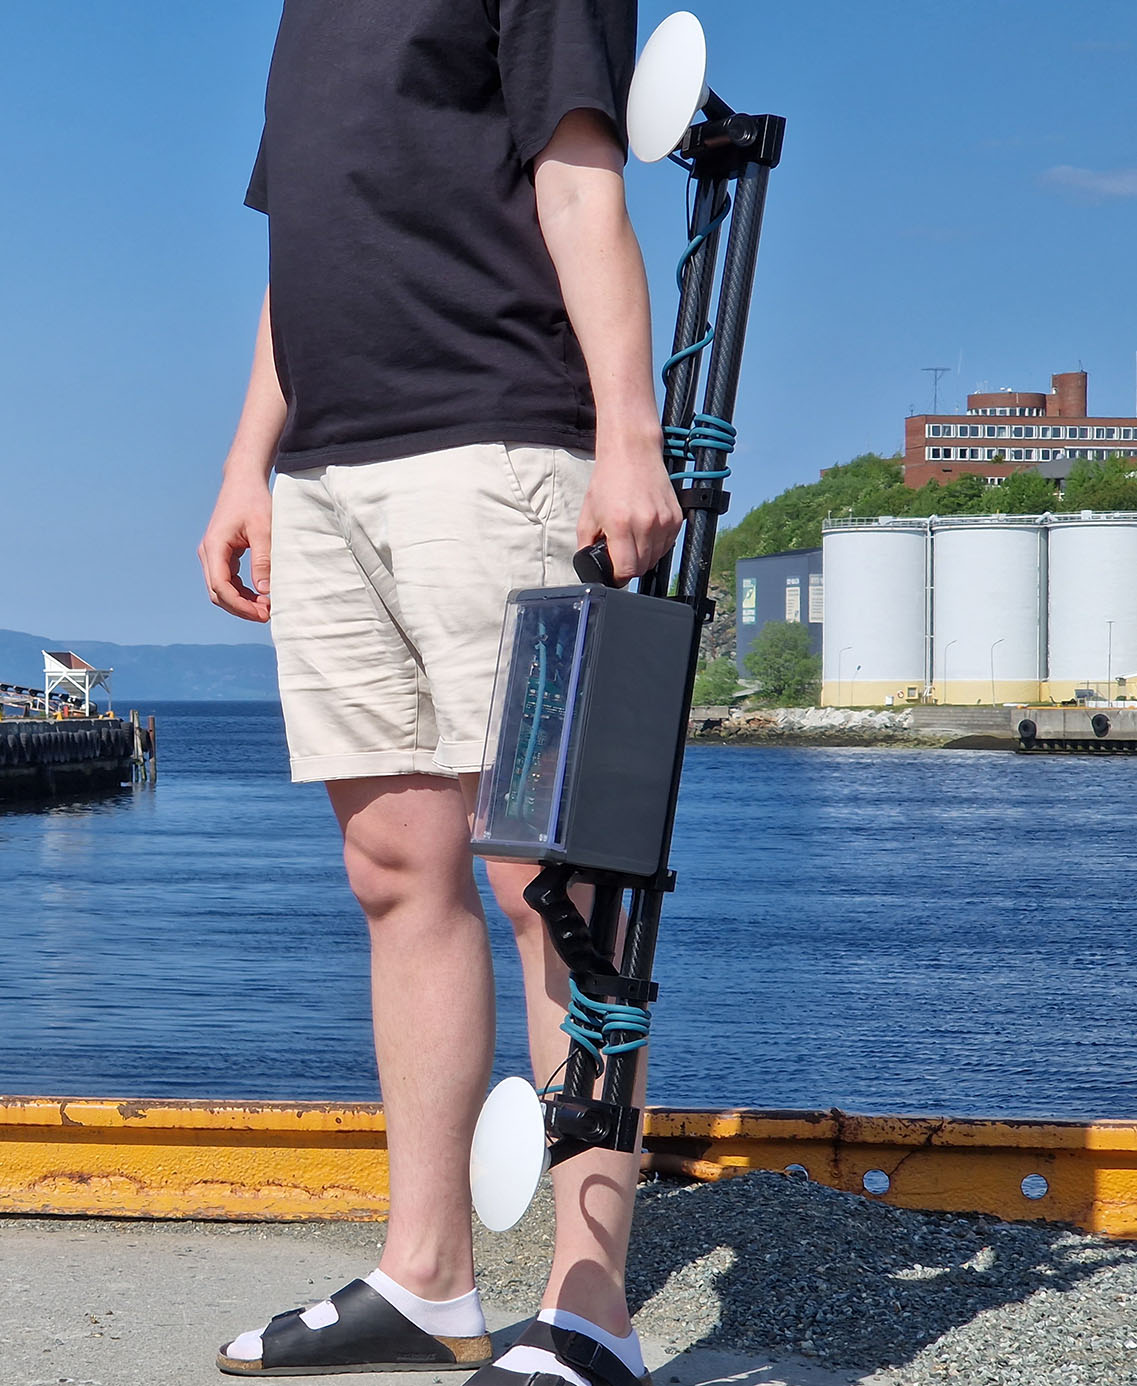
\includegraphics[width=\textwidth]{figures/ergonomics/resting.jpg}
    \caption{Depiction of the ample ground clearance when the \sr is carried in a relaxed left hand. The \sr not only excels in functionality but also makes a powerfull fashion statement when paired with socks and sandals.}
    \label{fig:egonomics_d}
\end{figure}



